\question (山东大学)在下列网络设备中,传输延迟最大的是
\par\twoch{局域网交换机}{网桥}{\textcolor{red}{路由器}}{集线器}
\begin{solution}由于路由器是网络层设备,在路由器上实现了物理层、数据链路层和网络层的功能,因此路由器的传输延迟时间是最大的。
\end{solution}
\question 某网络拓扑如下图所示,路由器R1只有到达子网192.168.1.0/24的路由。为使R1可以将IP分组正确地路由到图中所有子网,则在R1中需要增加的一条路由(目的网络,子网掩码,下一跳)是(
~)。

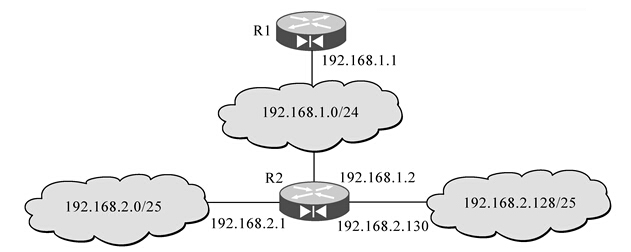
\includegraphics[width=3.33333in,height=1.33333in]{computerassets/68bb6dada2bc1a91fdc323c08ef13460.jpeg}
\par\fourch{192.168.2.0,255.255.255.128,192.168.1.1}{192.168.2.0,255.255.255.0,192.168.1.1}{192.168.2.0,255.255.255.128,192.168.1.2}{\textcolor{red}{192.168.2.0,255.255.255.0,192.168.1.2}}
\begin{solution}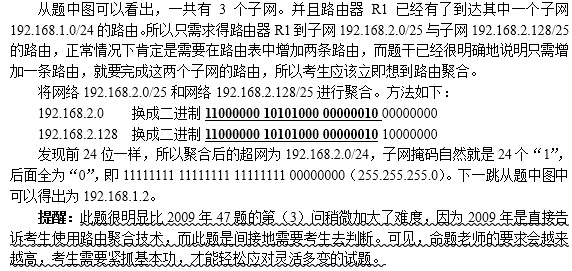
\includegraphics[width=3.33333in,height=1.58333in]{computerassets/587e0809d07702794990cae26f6745b2.jpeg}
\end{solution}
